\chapter{An introduction to Treewidth} \label{ch:treewidth}

The concept of tree decomposition and treewidth was first introduced by Robertson and Seymour to prove the famous graph minor theorem, which we state here for reference. 

% TODO: check if the statement is correct.
\begin{theorem}[Graph Minor Theorem, Robertson and Seymour \cite{robertson_seymour_1}]
	For any infinite sequence of graphs $G_1, G_2, \ldots$, there exist indices $i < j$ such that $G_i$ is a minor of $G_j$.
\end{theorem}

Treewidth later was proved to be very useful in many different areas of graph theory. 
As core algorithmic idea in this dissertation relies on treewidth, it is worth our effort to introduce treewidth and its properties in detail.

\section{Treewidth and its Elemetary Properties}

\begin{definition}[Tree Decomposition]
	Let $G$ be a finite graph and $V$ its vertex set. A \define{tree decomposition} of $G$ is a pair $(T, \{X_t\}_{t \in V(T)})$ where $T$ is a tree and $\{X_t\}_{t \in V(T)}$ is a family of subsets of $V$ (called bags) such that
	\begin{enumerate}
		\item $\bigcup_{t \in V(T)} X_t = V$,
		\item If vertices $u, v \in G$ are adjacent, there exists a $t \in T$  such that $u, v \in X_t$.
		\item Let $a, b$ be vertices of $T$. Since $T$ is a tree, there is a unique path connecting $a$ and $b$, which is denoted as $P$. If $v \in G$ and $v \in X_a, v \in X_b$, then for all $c \in P$, we have $v \in X_c$.
	\end{enumerate}

	Let $X_t$ be the bag such that $ \forall i \in T, |X_t| \geq |X_i|$ (That is, $X_t$ is the bag of the largest order). The \define{width} of the tree decomposition $(T, \{X_t\})$ is $|X_t| - 1$.
\end{definition}

\begin{definition}[Treewidth]
	The \define{tree width} of a graph $G$ is the minimum width over all of its tree decompositions.
\end{definition}

Tree decomposition requires the existence of a bag that contains all the adjacent vertices. 
If $u,v \in G$ and $\exists t$ such that $ u, v \in X_t $, however, it does not guarantee that $u$ and $v$ are adjacent in $G$.

\begin{example}[All graphs have a trivial tree decomposition]
	Let $G$ be a graph with vertex set $V$. Then $(T, \{X_t\})$ is a tree decomposition of $G$ where $T$ is a single node and $X_t = V$. The width of this tree decomposition is $|V| - 1$.

	Therefore, the treewidth of any graph $G$ is bounded above by $|V| - 1$.
	By Zorn's lemma, there must exist a tree decomposition of $G$ with minimum width.
\end{example}

Let us look at some examples of tree decomposition.

\begin{example}[Tree decomposition of a Tree]
	Let $G$ be a tree. We can construct a tree decomposition of $G$ in the following way.
	\begin{enumerate}
		\item Let each vertex of $G$ be a bag that contains only itself.
		\item On each edge of $G$, add a bag that contains the two endpoints of the edge.
	\end{enumerate}
	An example of this tree decomposition is shown in figure \ref{fig:tree_decomposition_of_tree}. 
	This gives the treewidth of a tree is $1$. 
	For any tree with at least one edge, there must be a bag that contains two or more vertices. This proves that the treewidth of a non-trivial tree is exactly $1$.
\end{example}

\begin{figure}[ht]
	\centering
	% Graph Board TikZ export
% Exported: 2026-08-10T20:25:43.207Z
% Title: Untitled Graph
% Nodes: 19, Edges: 15

\begingroup
% --- Colors (define-if-not-already-defined) ---
\providecolor{zxRed}{RGB}{232,165,165}   % X spiders
\providecolor{zxGreen}{RGB}{216,248,216} % Z spiders
\providecolor{zxYellow}{RGB}{255,255,0}     % hadamard 

\tikzset{
    EMPTY/.style={minimum size=3.4mm,
        outer sep=-1.7mm},
    DOT/.style={inner sep=0mm, minimum size=3.4mm, shape=circle,
        draw=black, outer sep=-0.5mm, line width=1pt},
    BLACK_DOT/.style={minimum size=2mm, inner sep=0.3mm,
        outer sep=-0.15mm, fill=black, shape=circle},
    WORD_BALL/.style={draw=black, shape=rectangle, minimum size=6.5mm,
        rounded corners=3.2mm, inner sep=1.2mm, outer sep=-1.0mm,
        scale=1, font={\large\boldmath}, line width=1pt},
    GREEN_DOT/.style={DOT, fill=zxGreen},
    GREEN_WORD_BALL/.style={WORD_BALL, fill=zxGreen},
    RED_DOT/.style={DOT, fill=zxRed},
    RED_WORD_BALL/.style={GREEN_WORD_BALL, fill=zxRed},
    YELLOW_BOX/.style={fill=zxYellow, draw=black, line width=1pt, shape=rectangle, inner sep=0.6mm,
        minimum height=3.4mm, minimum width=3.4mm,
        font={\large\boldmath}},
    EDGE/.style={draw=black, line width=1pt},
    BLUE_DASHED_EDGE/.style={EDGE, draw=blue, dashed}
}
\pgfdeclarelayer{edgelayer}
\pgfdeclarelayer{nodelayer}
\pgfsetlayers{edgelayer,nodelayer,main}

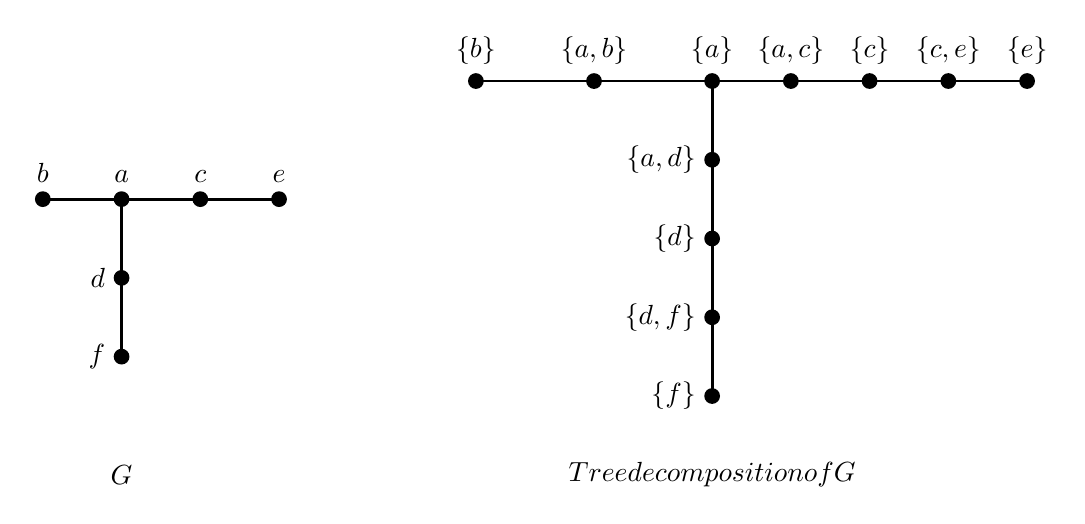
\begin{tikzpicture}
    \begin{pgfonlayer}{nodelayer}
        \node [label=above:{$a$}, BLACK_DOT] (1) at (-5.13158, 0.18421) {};
        \node [label=left:{$f$}, BLACK_DOT] (2) at (-5.13158, -1.81579) {};
        \node [label=above:{$b$}, BLACK_DOT] (3) at (-6.13158, 0.18421) {};
        \node [label=left:{$d$}, BLACK_DOT] (4) at (-5.13158, -0.81579) {};
        \node [label=above:{$c$}, BLACK_DOT] (5) at (-4.13158, 0.18421) {};
        \node [label=above:{$e$}, BLACK_DOT] (6) at (-3.13158, 0.18421) {};
        \node [EMPTY] (7) at (-5.13158, -3.31579) {$G$};
        \node [label=above:{$\{a\}$}, BLACK_DOT] (8) at (2.36842, 1.68421) {};
        \node [label=left:{$\{d\}$}, BLACK_DOT] (9) at (2.36842, -0.31579) {};
        \node [label=above:{$\{a,b\}$}, BLACK_DOT] (10) at (0.86842, 1.68421) {};
        \node [label=left:{$\{a,d\}$}, BLACK_DOT] (11) at (2.36842, 0.68421) {};
        \node [label=above:{$\{a, c\}$}, BLACK_DOT] (12) at (3.36842, 1.68421) {};
        \node [label=above:{$\{c\}$}, BLACK_DOT] (13) at (4.36842, 1.68421) {};
        \node [label=above:{$\{b\}$}, BLACK_DOT] (14) at (-0.63158, 1.68421) {};
        \node [label=left:{$\{d, f\}$}, BLACK_DOT] (15) at (2.36842, -1.31579) {};
        \node [label=left:{$\{f\}$}, BLACK_DOT] (16) at (2.36842, -2.31579) {};
        \node [label=above:{$\{c,e\}$}, BLACK_DOT] (17) at (5.36842, 1.68421) {};
        \node [label=above:{$\{e\}$}, BLACK_DOT] (18) at (6.36842, 1.68421) {};
        \node [EMPTY] (19) at (2.36842, -3.31579) {$\text{Tree decomposition of } G$};
    \end{pgfonlayer}
    \begin{pgfonlayer}{edgelayer}
        \draw[EDGE] (3) to (1);
        \draw[EDGE] (4) to (1);
        \draw[EDGE] (5) to (1);
        \draw[EDGE] (2) to (4);
        \draw[EDGE] (6) to (5);
        \draw[EDGE] (10) to (8);
        \draw[EDGE] (11) to (8);
        \draw[EDGE] (12) to (8);
        \draw[EDGE] (9) to (11);
        \draw[EDGE] (13) to (12);
        \draw[EDGE] (14) to (10);
        \draw[EDGE] (16) to (15);
        \draw[EDGE] (9) to (15);
        \draw[EDGE] (18) to (17);
        \draw[EDGE] (17) to (13);
    \end{pgfonlayer}
\end{tikzpicture}

\endgroup
	\caption{A tree decomposition of a tree.}
	\label{fig:tree_decomposition_of_tree}
\end{figure}

\begin{example}[Tree Decomposition of Some Random Graphs]
	See figure \ref{fig:tree_decomposition_of_random_graph} for an example of a tree decomposition of a triangulated graph.
\end{example}

\begin{figure}[ht]
	\centering
	% Graph Board TikZ export
% Exported: 2026-08-10T21:07:29.267Z
% Title: Untitled Graph
% Nodes: 15, Edges: 15

\begingroup
% --- Colors (define-if-not-already-defined) ---
\providecolor{zxRed}{RGB}{232,165,165}   % X spiders
\providecolor{zxGreen}{RGB}{216,248,216} % Z spiders
\providecolor{zxYellow}{RGB}{255,255,0}     % hadamard 

\tikzset{
    EMPTY/.style={minimum size=3.4mm,
        outer sep=-1.7mm},
    DOT/.style={inner sep=0mm, minimum size=3.4mm, shape=circle,
        draw=black, outer sep=-0.5mm, line width=1pt},
    BLACK_DOT/.style={minimum size=2mm, inner sep=0.3mm,
        outer sep=-0.15mm, fill=black, shape=circle},
    WORD_BALL/.style={draw=black, shape=rectangle, minimum size=6.5mm,
        rounded corners=3.2mm, inner sep=1.2mm, outer sep=-1.0mm,
        scale=1, font={\large\boldmath}, line width=1pt},
    GREEN_DOT/.style={DOT, fill=zxGreen},
    GREEN_WORD_BALL/.style={WORD_BALL, fill=zxGreen},
    RED_DOT/.style={DOT, fill=zxRed},
    RED_WORD_BALL/.style={GREEN_WORD_BALL, fill=zxRed},
    YELLOW_BOX/.style={fill=zxYellow, draw=black, line width=1pt, shape=rectangle, inner sep=0.6mm,
        minimum height=3.4mm, minimum width=3.4mm,
        font={\large\boldmath}},
    EDGE/.style={draw=black, line width=1pt},
    BLUE_DASHED_EDGE/.style={EDGE, draw=blue, dashed}
}
\pgfdeclarelayer{edgelayer}
\pgfdeclarelayer{nodelayer}
\pgfsetlayers{edgelayer,nodelayer,main}

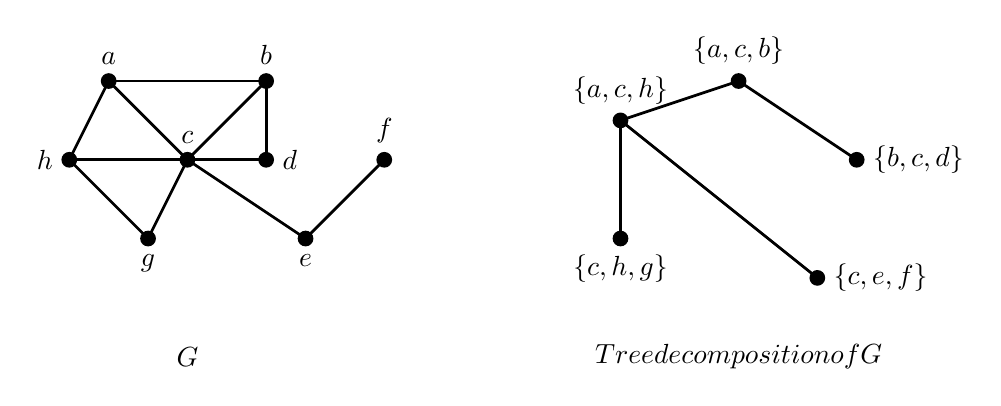
\begin{tikzpicture}
    \begin{pgfonlayer}{nodelayer}
        \node [EMPTY] (1) at (-2.96667, -2.1) {$G$};
        \node [EMPTY] (2) at (4.03333, -2.1) {$\text{Tree decomposition of } G$};
        \node [label=above:{$a$}, BLACK_DOT] (3) at (-3.96667, 1.4) {};
        \node [label=left:{$h$}, BLACK_DOT] (4) at (-4.46667, 0.4) {};
        \node [label=below:{$g$}, BLACK_DOT] (5) at (-3.46667, -0.6) {};
        \node [label=below:{$e$}, BLACK_DOT] (6) at (-1.46667, -0.6) {};
        \node [label=above:{$f$}, BLACK_DOT] (7) at (-0.46667, 0.4) {};
        \node [label=above:{$b$}, BLACK_DOT] (8) at (-1.96667, 1.4) {};
        \node [label=right:{$d$}, BLACK_DOT] (9) at (-1.96667, 0.4) {};
        \node [label=above:{$c$}, BLACK_DOT] (10) at (-2.96667, 0.4) {};
        \node [label=below:{$\{c,h, g\}$}, BLACK_DOT] (11) at (2.53333, -0.6) {};
        \node [label=above:{$\{a,c,h\}$}, BLACK_DOT] (12) at (2.53333, 0.9) {};
        \node [label=above:{$\{a,c,b\}$}, BLACK_DOT] (13) at (4.03333, 1.4) {};
        \node [label=right:{$\{b, c, d\}$}, BLACK_DOT] (14) at (5.53333, 0.4) {};
        \node [label=right:{$\{c,e,f\}$}, BLACK_DOT] (15) at (5.03333, -1.1) {};
    \end{pgfonlayer}
    \begin{pgfonlayer}{edgelayer}
        \draw[EDGE] (3) to (10);
        \draw[EDGE] (4) to (10);
        \draw[EDGE] (3) to (4);
        \draw[EDGE] (5) to (10);
        \draw[EDGE] (4) to (5);
        \draw[EDGE] (3) to (8);
        \draw[EDGE] (10) to (8);
        \draw[EDGE] (8) to (9);
        \draw[EDGE] (6) to (7);
        \draw[EDGE] (10) to (9);
        \draw[EDGE] (10) to (6);
        \draw[EDGE] (11) to (12);
        \draw[EDGE] (13) to (12);
        \draw[EDGE] (13) to (14);
        \draw[EDGE] (15) to (12);
    \end{pgfonlayer}
\end{tikzpicture}

\endgroup

	\caption{A tree decomposition of a triangulated graph.}
	\label{fig:tree_decomposition_of_random_graph}
\end{figure}

The following lemma will be useful.

\begin{lemma}
	Let $G$ be a graph and $T$ its tree decomposition of at least three vertices. Let $a \in T$.
	If deleting $a$ from $T$ produces at least two subgraphs of $T$, which we label as $C_1, C_2$, that are disconnected, then the subgraph of $G$ induced by the vertices in $\bigcup_{t\in C_1} \{X_t\} - A $ and $\bigcup_{t\in C_2} \{X_t\} - A $ are disconnected.
\end{lemma} \label{lem:tree_decomposition_disconnected_subgraph}

\begin{proof}
	It is sufficient to show that for all $v\in G_1$ and $u \in G_2$, $v$ is not adjacent to $u$. 

	Assume that $v \in G_1$ and $u \in G_2$ and they are adjacent. 
	Let $v \in X_s$, $u \in X_r$, and let $P_0$ be the unique path from $s$ to $r$ in $T$. By our assumption, $P_0$ contains the point $a$.

	By property 2 of tree decomposition, there exists $t \in T$ such that $v, u \in X_t$.
	Since $T$ is connected, there exists a path $P_1$ from $s$ to $t$ and path $P_2$ from $r$ to $t$.
	If none of them pass through $a$, then there is a cycle in $T$ consisting of $P_0$, $P_1$, and $P_2$. This contradicts the fact that $T$ is a tree. Therefore, at least one of them must pass through $a$.

	Without loss of any generality, let $P_1$ pass through $a$.
	By property 3 of tree decomposition, $P_1$ is a path whose endpoints are bags that contain $v$, so by property 3 again the bag $X_a$ contains $v$ as well.
	This is a contradiction to the assumption that $v \in G_1$. (Recall that $G_1$ does not contain any vertices that are in $X_a$)
\end{proof}

\begin{example}[Treewidth of a Complete Graph]
	The treewidth of a complete graph $K_n$ is $n-1$, as all tree decompositions of $K_n$ must contain a bag that contains all vertices of $K_n$.

	To prove this claim, assume $T$ is a tree decomposition of $K_n$ and let $X_i$ be the largest bag of $T$ that does not contain all vertices of $K_n$. 
	Since $X_i$ does not contain all vertices of $K_n$, there exists a vertex $v \in K_n$ such that $v \notin X_i$, which is in the bag $X_j$ for some $j$. Again, as $v$ is connected to all other vertices and $X_j$ does not contain all vertices, there must be a third bag in $T$. 

	In a tree with at least three vertices, there must exist a vertex $a$ such that deleting $a$ from $T$ will produce at least two disconnected subgraphs of $T$.
	Now we can invoke lemma \ref{lem:tree_decomposition_disconnected_subgraph} , which states that deleting $a$ from $T$ will produce at least two disconnected subgraphs of $T$. This is not possible as $K_n$ is a complete graph, so all vertices are connected. 

	Therefore, all tree decompositions of $K_n$ must contain a bag that contains all vertices of $K_n$, which proves the claim.
\end{example}

If graph $G$ is a minor of $H$, then the treewidth of $G$ is less than or equal to the treewidth of $H$.
The definition of graph minor is presented here for reference.

\begin{definition}[Graph Minor]
	Let $G$ and $H$ be two graphs. We say that $G$ is a \define{minor} of $H$ if $G$ can be obtained from $H$ by a sequence of the following operations:
	\begin{enumerate}
		\item Deleting an edge,
		\item Deleting a vertex,
		\item Contracting an edge.
	\end{enumerate}
	The process of contracting an edge $e = (u, v)$ is to delete the edge $e$ and merge the two vertices $u$ and $v$ into a single vertex $w$. The new vertex $w$ is adjacent to all the neighbors of $u$ and $v$.
\end{definition}

\begin{lemma}[Graph Minor and Treewidth]\label{lem:minor_treewidth}
	Let $G$ and $H$ be two graphs. If $G$ is a minor of $H$, then the treewidth of $G$ is less than or equal to the treewidth of $H$.
\end{lemma}

The proof of this lemma is presented in section \ref{sec:proofs}.

We can use lemma \ref{lem:minor_treewidth} to prove various lower bounds on the treewidth. 

\begin{corollary}\label{cor:treewidth_delta_lower_bound}
	Let $\delta$ be the minimum vertex degree of a graph $G$. The treewidth of $G$ is at least $\delta$.
\end{corollary}

\begin{proof}
	We can continuously contract edges in $G$ until we obtain a complete graph $K_{\delta + 1}$. By lemma \ref{lem:minor_treewidth}, the treewidth of $G$ is at least the treewidth of $K_{\delta + 1}$, which is $\delta$.
\end{proof}

Using these lemmas, we can find the treewidth of more complicated graphs.

\begin{example}
	The treewidth of a circle graph is $2$.
	By corollary \ref{cor:treewidth_delta_lower_bound}, the treewidth of a circle graph is at least $2$ as the minimum vertex degree of a circle graph is $2$.
	We can construct a tree decomposition of a circle graph with width $2$ as follows.

	Let vertex $a$ be the start of the cycle. Delete one edge next to $a$ and treat the rest of the graph as a tree, with the maximum bag of size $2$.
	Adding $a$ to all bags of the tree decomposition gives a tree decomposition of the circle graph with bags of maximum size $3$ and width $2$.

	See figure \ref{fig:tree_decomposition_of_circle_graph} for an example.
\end{example}

\begin{figure}[ht]
	\centering
	% Graph Board TikZ export
% Exported: 2026-08-11T21:10:27.536Z
% Title: Untitled Graph
% Nodes: 12, Edges: 11

\begingroup
% --- Colors (define-if-not-already-defined) ---
\providecolor{zxRed}{RGB}{232,165,165}   % X spiders
\providecolor{zxGreen}{RGB}{216,248,216} % Z spiders
\providecolor{zxYellow}{RGB}{255,255,0}     % hadamard 
\providecolor{zxBlue}{RGB}{68,126,255}     % hadamard 


\tikzset{
    EMPTY/.style={minimum size=3.4mm,
        outer sep=-1.7mm},
    DOT/.style={inner sep=0mm, minimum size=3.4mm, shape=circle,
        draw=black, outer sep=-0.5mm, line width=1pt},
    BLACK_DOT/.style={minimum size=2mm, inner sep=0.3mm,
        outer sep=-0.15mm, fill=black, shape=circle},
    WORD_BALL/.style={draw=black, shape=rectangle, minimum size=6.5mm,
        rounded corners=3.2mm, inner sep=1.2mm, outer sep=-1.0mm,
        scale=1, font={\large\boldmath}, line width=1pt},
    GREEN_DOT/.style={DOT, fill=zxGreen},
    GREEN_WORD_BALL/.style={WORD_BALL, fill=zxGreen},
    RED_DOT/.style={DOT, fill=zxRed},
    RED_WORD_BALL/.style={GREEN_WORD_BALL, fill=zxRed},
    YELLOW_BOX/.style={fill=zxYellow, draw=black, line width=1pt, shape=rectangle, inner sep=0.6mm,
        minimum height=3.4mm, minimum width=3.4mm,
        font={\large\boldmath}},
    EDGE/.style={draw=black, line width=1pt},
    BLUE_DASHED_EDGE/.style={-, dashed, dash pattern=on 2pt off 0.5pt, ultra thick, zxBlue}
}
\pgfdeclarelayer{edgelayer}
\pgfdeclarelayer{nodelayer}
\pgfsetlayers{edgelayer,nodelayer,main}

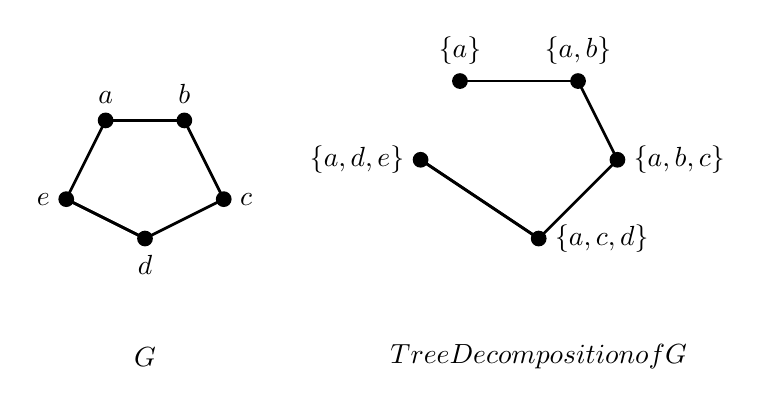
\begin{tikzpicture}
    \begin{pgfonlayer}{nodelayer}
        \node [label=above:{$b$}, BLACK_DOT] (1) at (-1.91667, 0.91667) {};
        \node [label=above:{$a$}, BLACK_DOT] (2) at (-2.91667, 0.91667) {};
        \node [label=left:{$e$}, BLACK_DOT] (3) at (-3.41667, -0.08333) {};
        \node [label=below:{$d$}, BLACK_DOT] (4) at (-2.41667, -0.58333) {};
        \node [label=right:{$c$}, BLACK_DOT] (5) at (-1.41667, -0.08333) {};
        \node [label=right:{$\{a, b, c\}$}, BLACK_DOT] (6) at (3.58333, 0.41667) {};
        \node [label=above:{$\{a, b\}$}, BLACK_DOT] (7) at (3.08333, 1.41667) {};
        \node [label=left:{$\{a, d, e\}$}, BLACK_DOT] (8) at (1.08333, 0.41667) {};
        \node [label=right:{$\{a, c, d\}$}, BLACK_DOT] (9) at (2.58333, -0.58333) {};
        \node [label=above:{$\{a\}$}, BLACK_DOT] (10) at (1.58333, 1.41667) {};
        \node [EMPTY] (11) at (-2.41667, -2.08333) {$G$};
        \node [EMPTY] (12) at (2.58333, -2.08333) {$\text{Tree Decomposition of }G$};
    \end{pgfonlayer}
    \begin{pgfonlayer}{edgelayer}
        \draw[EDGE] (1) to (2);
        \draw[EDGE] (2) to (3);
        \draw[EDGE] (3) to (4);
        \draw[EDGE] (1) to (5);
        \draw[EDGE] (5) to (4);
        \draw[EDGE] (6) to (7);
        \draw[EDGE] (6) to (9);
        \draw[EDGE] (9) to (8);
        \draw[EDGE] (4) to (3);
        \draw[EDGE] (8) to (9);
        \draw[EDGE] (10) to (7);
    \end{pgfonlayer}
\end{tikzpicture}

\endgroup
	\caption{A tree decomposition of a circle graph.}
	\label{fig:tree_decomposition_of_circle_graph}
\end{figure}

\section{Traingulated Graphs and Treewidth}

Treewidth is closely related to triangulated graphs, as we shall explain in this section.

\begin{definition}[Triangulated Graph]
	A graph $G$ is \define{triangulated} if every cycle of length greater than or equal to $4$ has a chord.
	A chord is an edge that connects two non-adjacent vertices in the cycle.
	Triangulated graphs are also called \define{chordal graphs}.
\end{definition}

The triangulation properties is a subtle requirement for connections between vertices. 
In one sense no two vertices are far away from each other if and only if there is a loop connecting them. 

Figure show examples of two triangulated graphs. All trees and complete graphs are triangulated. 
Cycle of length greater than three are not. 
Unions of triangles are not garanteed to be triangulated.
See figure \ref{fig:triangulated_example} for examples of triangulated and non-triangulated graphs.

\begin{figure}[ht]
	\centering
	% Graph Board TikZ export
% Exported: 2026-08-14T19:30:41.123Z
% Title: Untitled Graph
% Nodes: 29, Edges: 38

\begingroup
% --- Colors (define-if-not-already-defined) ---
\providecolor{zxRed}{RGB}{232,165,165}   % X spiders
\providecolor{zxGreen}{RGB}{216,248,216} % Z spiders
\providecolor{zxYellow}{RGB}{255,255,0}     % hadamard 
\providecolor{zxBlue}{RGB}{68,126,255}     % hadamard 


\tikzset{
    EMPTY/.style={minimum size=3.4mm,
        outer sep=-1.7mm},
    DOT/.style={inner sep=0mm, minimum size=3.4mm, shape=circle,
        draw=black, outer sep=-0.5mm, line width=1pt},
    BLACK_DOT/.style={minimum size=2mm, inner sep=0.3mm,
        outer sep=-0.15mm, fill=black, shape=circle},
    WORD_BALL/.style={draw=black, shape=rectangle, minimum size=6.5mm,
        rounded corners=3.2mm, inner sep=1.2mm, outer sep=-1.0mm,
        scale=1, font={\large\boldmath}, line width=1pt},
    GREEN_DOT/.style={DOT, fill=zxGreen},
    GREEN_WORD_BALL/.style={WORD_BALL, fill=zxGreen},
    RED_DOT/.style={DOT, fill=zxRed},
    RED_WORD_BALL/.style={GREEN_WORD_BALL, fill=zxRed},
    YELLOW_BOX/.style={fill=zxYellow, draw=black, line width=1pt, shape=rectangle, inner sep=0.6mm,
        minimum height=3.4mm, minimum width=3.4mm,
        font={\large\boldmath}},
    EDGE/.style={draw=black, line width=1pt},
    BLUE_DASHED_EDGE/.style={-, dashed, dash pattern=on 2pt off 0.5pt, ultra thick, zxBlue},
    GRAY_DASHED_EDGE/.style={-, dashed, dash pattern=on 3pt off 1.5pt, thick, lightgray}
}
\pgfdeclarelayer{edgelayer}
\pgfdeclarelayer{nodelayer}
\pgfsetlayers{edgelayer,nodelayer,main}

\begin{tikzpicture}
    \begin{pgfonlayer}{nodelayer}
        \node [BLACK_DOT] (1) at (-4.84483, 1.67241) {};
        \node [BLACK_DOT] (2) at (-3.84483, 1.67241) {};
        \node [BLACK_DOT] (3) at (-2.84483, 1.67241) {};
        \node [BLACK_DOT] (4) at (-0.84483, 1.67241) {};
        \node [BLACK_DOT] (5) at (-1.84483, 1.67241) {};
        \node [BLACK_DOT] (6) at (1.15517, -1.32759) {};
        \node [BLACK_DOT] (7) at (1.65517, -1.82759) {};
        \node [BLACK_DOT] (8) at (2.15517, -1.32759) {};
        \node [BLACK_DOT] (9) at (3.15517, -1.32759) {};
        \node [BLACK_DOT] (10) at (2.65517, -1.82759) {};
        \node [BLACK_DOT] (11) at (1.15517, -0.82759) {};
        \node [BLACK_DOT] (12) at (1.65517, -0.32759) {};
        \node [BLACK_DOT] (13) at (2.65517, -0.32759) {};
        \node [BLACK_DOT] (14) at (2.15517, -0.82759) {};
        \node [BLACK_DOT] (15) at (3.15517, -0.82759) {};
        \node [BLACK_DOT] (16) at (-2.84483, 2.67241) {};
        \node [EMPTY] (17) at (-2.84483, 0.67241) {$\text{tree}$};
        \node [EMPTY] (18) at (2.15517, 0.67241) {$\text{clique}$};
        \node [EMPTY] (19) at (2.15517, -2.82759) {$\text{Non Triangulated}$};
        \node [BLACK_DOT] (20) at (-3.84483, -0.82759) {};
        \node [BLACK_DOT] (21) at (-3.84483, -1.82759) {};
        \node [BLACK_DOT] (22) at (-2.84483, -1.82759) {};
        \node [BLACK_DOT] (23) at (-2.84483, -0.82759) {};
        \node [EMPTY] (24) at (-3.34483, -2.82759) {$\text{Non Triangulated}$};
        \node [BLACK_DOT] (25) at (2.15517, 2.67241) {};
        \node [BLACK_DOT] (26) at (1.15517, 2.17241) {};
        \node [BLACK_DOT] (27) at (1.65517, 1.17241) {};
        \node [BLACK_DOT] (28) at (2.65517, 1.17241) {};
        \node [BLACK_DOT] (29) at (3.15517, 2.17241) {};
    \end{pgfonlayer}
    \begin{pgfonlayer}{edgelayer}
        \draw[EDGE] (4) to (5);
        \draw[EDGE] (5) to (3);
        \draw[EDGE] (3) to (2);
        \draw[EDGE] (2) to (1);
        \draw[BLUE_DASHED_EDGE] (9) to (10);
        \draw[EDGE] (10) to (8);
        \draw[EDGE] (8) to (7);
        \draw[BLUE_DASHED_EDGE] (7) to (6);
        \draw[EDGE] (6) to (8);
        \draw[BLUE_DASHED_EDGE] (7) to (10);
        \draw[EDGE] (8) to (9);
        \draw[EDGE] (13) to (14);
        \draw[EDGE] (14) to (12);
        \draw[BLUE_DASHED_EDGE] (12) to (11);
        \draw[EDGE] (11) to (14);
        \draw[BLUE_DASHED_EDGE] (12) to (13);
        \draw[BLUE_DASHED_EDGE] (11) to (6);
        \draw[EDGE] (14) to (8);
        \draw[EDGE] (8) to (11);
        \draw[BLUE_DASHED_EDGE] (13) to (15);
        \draw[EDGE] (15) to (14);
        \draw[EDGE] (14) to (9);
        \draw[BLUE_DASHED_EDGE] (15) to (9);
        \draw[EDGE] (16) to (3);
        \draw[BLUE_DASHED_EDGE] (20) to (23);
        \draw[BLUE_DASHED_EDGE] (21) to (22);
        \draw[BLUE_DASHED_EDGE] (22) to (23);
        \draw[BLUE_DASHED_EDGE] (20) to (21);
        \draw[EDGE] (26) to (29);
        \draw[EDGE] (26) to (25);
        \draw[EDGE] (25) to (29);
        \draw[EDGE] (27) to (26);
        \draw[EDGE] (28) to (26);
        \draw[EDGE] (27) to (25);
        \draw[EDGE] (28) to (25);
        \draw[EDGE] (27) to (29);
        \draw[EDGE] (28) to (29);
        \draw[EDGE] (27) to (28);
    \end{pgfonlayer}
\end{tikzpicture}

\endgroup
	\caption{Examples of two triangulated graphs (tree and clique) and two non-triangulated graphs (cycle and union of triangles).
	The chordless cycles of non-triangulated graphs are dashed in blue.}
	\label{fig:triangulated_example}
\end{figure}

\begin{lemma}[Removing a Vertex from Triangualted Graph]\label{lem:eleminate_vertex_triangulated}
	Let $G$ be a triangulated graph and $v$ any vertex in $G$. Then the graph $G \setminus \{v\}$ is triangulated.
	Note $G \setminus \{v\}$ is the graph induced from the vertex set $V(G) \setminus \{v\}$.
\end{lemma}

\begin{proof}
	If $G\setminus \{v\}$ is not triangulated, then there exists a cycle of length greater than or equal to $4$ in $G\setminus \{v\}$ that does not have a chord.
	The same cycle exists in $G$ and does not have a chord, meaning $G$ is not triangulated either.
	This concludes the proof by contraposition.
\end{proof}

The following lemma follows by induction. 

\begin{lemma}[Induced Subgraph of Triangulated Graph is Triangulated]
	Let $G$ be a triangulated graph and $H$ an induced subgraph of $G$. Then $H$ is triangulated.
\end{lemma}

\begin{definition}[Simplicial Vertex]
	A vertex $v$ in a graph $G$ is \define{simplicial} if the subgraph induced by the neighbors of $v$ is a complete graph.
\end{definition}

\begin{lemma}[Existence of Simplicial Vertex in Triangulated Graphs]\label{lem:simplicial_vertex}
	Every triangulated graph has at least one simplicial vertex.
\end{lemma}

The proof of this lemma is presented in section \ref{sec:proofs}.

\begin{definition}[Perfect Elimination Ordering]
	A \define{perfect elimination ordering} of a graph $G$ is an ordering of the vertices $[v_1, v_2, \ldots, v_n]$ such that each vertex $v_i$ is simplical in the subgraph induced by $[v_i, v_{i+1}, \ldots, v_n]$.
\end{definition}

The reason is its called a perfect elimination is that $v_1$ is a simplical vertex in $G$, $v_2$ is a simplicial vertex in $G \setminus \{v_1\}$ (that is graph $G$ with vertex $v_1$ removed), and so on.
An example of perfect elimination order of a triangualted graph is shown in figure \ref{fig:perfect_elimination_ordering}.

\begin{figure}[ht]
	\centering
	% Graph Board TikZ export
% Exported: 2026-08-14T20:17:40.816Z
% Title: Untitled Graph
% Nodes: 17, Edges: 19

\begingroup
% --- Colors (define-if-not-already-defined) ---
\providecolor{zxRed}{RGB}{232,165,165}   % X spiders
\providecolor{zxGreen}{RGB}{216,248,216} % Z spiders
\providecolor{zxYellow}{RGB}{255,255,0}     % hadamard 
\providecolor{zxBlue}{RGB}{68,126,255}     % hadamard 


\tikzset{
    EMPTY/.style={minimum size=3.4mm,
        outer sep=-1.7mm},
    DOT/.style={inner sep=0mm, minimum size=3.4mm, shape=circle,
        draw=black, outer sep=-0.5mm, line width=1pt},
    BLACK_DOT/.style={minimum size=2mm, inner sep=0.3mm,
        outer sep=-0.15mm, fill=black, shape=circle},
    WORD_BALL/.style={draw=black, shape=rectangle, minimum size=6.5mm,
        rounded corners=3.2mm, inner sep=1.2mm, outer sep=-1.0mm,
        scale=1, font={\large\boldmath}, line width=1pt},
    GREEN_DOT/.style={DOT, fill=zxGreen},
    GREEN_WORD_BALL/.style={WORD_BALL, fill=zxGreen},
    RED_DOT/.style={DOT, fill=zxRed},
    RED_WORD_BALL/.style={GREEN_WORD_BALL, fill=zxRed},
    YELLOW_BOX/.style={fill=zxYellow, draw=black, line width=1pt, shape=rectangle, inner sep=0.6mm,
        minimum height=3.4mm, minimum width=3.4mm,
        font={\large\boldmath}},
    EDGE/.style={draw=black, line width=1pt},
    BLUE_DASHED_EDGE/.style={-, dashed, dash pattern=on 2pt off 0.5pt, ultra thick, zxBlue},
    GRAY_DASHED_EDGE/.style={-, dashed, dash pattern=on 3pt off 1.5pt, thick, lightgray}
}
\pgfdeclarelayer{edgelayer}
\pgfdeclarelayer{nodelayer}
\pgfsetlayers{edgelayer,nodelayer,main}

\begin{tikzpicture}
    \begin{pgfonlayer}{nodelayer}
        \node [BLACK_DOT] (1) at (-4.67647, 0.79412) {};
        \node [BLACK_DOT] (2) at (-5.67647, 0.29412) {};
        \node [RED_DOT] (3) at (-5.17647, -0.70588) {};
        \node [BLACK_DOT] (4) at (-4.17647, -0.70588) {};
        \node [BLACK_DOT] (5) at (-3.67647, 0.29412) {};
        \node [BLACK_DOT] (6) at (-0.67647, 0.79412) {};
        \node [RED_DOT] (7) at (-1.67647, 0.29412) {};
        \node [BLACK_DOT] (8) at (-0.17647, -0.70588) {};
        \node [BLACK_DOT] (9) at (0.32353, 0.29412) {};
        \node [RED_DOT] (10) at (2.82353, 0.79412) {};
        \node [BLACK_DOT] (11) at (3.32353, -0.70588) {};
        \node [BLACK_DOT] (12) at (3.82353, 0.29412) {};
        \node [BLACK_DOT] (13) at (5.82353, -0.70588) {};
        \node [BLACK_DOT] (14) at (6.32353, 0.29412) {};
        \node [EMPTY] (15) at (-2.67647, -0.20588) {$\rightarrow$};
        \node [EMPTY] (16) at (1.32353, -0.20588) {$\rightarrow$};
        \node [EMPTY] (17) at (4.82353, -0.20588) {$\rightarrow$};
    \end{pgfonlayer}
    \begin{pgfonlayer}{edgelayer}
        \draw[EDGE] (2) to (5);
        \draw[EDGE] (2) to (1);
        \draw[EDGE] (1) to (5);
        \draw[EDGE] (3) to (2);
        \draw[EDGE] (4) to (2);
        \draw[EDGE] (4) to (1);
        \draw[EDGE] (3) to (5);
        \draw[EDGE] (4) to (5);
        \draw[EDGE] (3) to (4);
        \draw[EDGE] (7) to (9);
        \draw[EDGE] (7) to (6);
        \draw[EDGE] (6) to (9);
        \draw[EDGE] (8) to (7);
        \draw[EDGE] (8) to (6);
        \draw[EDGE] (8) to (9);
        \draw[EDGE] (10) to (12);
        \draw[EDGE] (11) to (10);
        \draw[EDGE] (11) to (12);
        \draw[EDGE] (13) to (14);
    \end{pgfonlayer}
\end{tikzpicture}

\endgroup
	\caption{Perfect elimination ordering of a triangulated graph. The simplical vertices at each step of elimination are colored in red. }
	\label{fig:perfect_elimination_ordering}
\end{figure}

\begin{theorem}[Triangulated Graph and Perfect Elimination Ordering]\label{thm:triangulated_perfect_elimination_ordering}
	A graph $G$ is triangulated if and only if it has a perfect elimination ordering.
\end{theorem}

\begin{proof}
	Sufficient condition. Assuming $G$ has a perfect elimination ordering $[v_1, v_2, \ldots, v_n]$. Let $P$ be a cycle of length greater than 3.
	Among the vertice in $P$, one of them is ordered first in the perfect elimination ordering, say $v_i$.
	$v_i$ connects to at least two othere vertices in $P$. Since $v_i$ is simplicial in the subgraph induced by $[v_i, v_{i+1}, \ldots, v_n]$, there must be a chord in $P$ that connects two non-adjacent vertices in $P$. Therefore, $G$ is triangulated.

	The necessary condiation can be proved by induction on the number of vertices in $G$ using lemma \ref{lem:simplicial_vertex}.
	
	The base case is when $G$ has only one vertex, which is trivially simplicial.

	Let $G$ be a triangulated graph $n$ vertices. By lemma \ref{lem:simplicial_vertex}, there exists a simplicial vertex $v$ in $G$.
	Elimination of $v$ gives $G \ v$ with $n-1$ vertices. 
	$G\setminus \{v\}$ is triangulated by lemma \ref{lem:eleminate_vertex_triangulated}. So the proof is done by induction.
\end{proof}

\subsection{Treewidth and Triangulated Graphs}

Recall that an induced subgraph of a graph $G$ is a graph formed from a subset of the vertices of $G$ and all of the edges connecting pairs of vertices in that subset.
Using the notion of induced subgraph, we have the following important theorem that connects treewidth and triangulated graphs.

\begin{theorem}[Treewidth and Triangulated Graph]\label{thm:treewidth_triangulated_graph}
	For all graph $G$, there exists a triangulated graph $T$ such that $G$ is the induced subgraph of $T$ and $\text{tw}(G) = \text{tw}(T)$.
\end{theorem}

\begin{proof}
	Let $G$ be a graph. It is sufficient to show that for all tree decomposition of $G$, which we label as $T$, there exists a triangulated graph $F$ with the same tree decomposition and $G$ is the induced subgraph of $F$.
	We shall give a constructive proof.

	We can construct the triangulated graph $F$ from $G$ in the following steps.
    \begin{enumerate}
    	\item Let $X_l$ be a leaf in $T$. \footnote{A leaf is a vertex in a tree with degree 1.} Let $X_p$ be the parent of $X_l$ in $T$.
		   	We assume that $X_l \setminus X_p$ is a set of one element (justified later).
		\item Let $v$ be the unique vertex in $X_l \setminus X_p$. No other bags in $T$ contain $v$. If there is another bag that contains $v$, the path from $X_l$ to that bag must pass through $X_p$, and $X_p$ must contain $v$ by property 3 of tree decomposition. This is a contradiction to the assumption that $v \notin X_p$.
		\item In graph $F$, let $v$ has neighbours to all the vertices in $X_l$, and let the subgraph induced by $X_l$ be a complete graph.
		\item Remove $X_l$ from $T$ and repeat the process until $T$ contain only one bag. Make the vertices in this bag a clique. As the graph $G$ is finite, this process must terminate.
    \end{enumerate}

	This process will produce a perfect elimination ordering of $F$ and therefore $F$ is triangulated.
	The original tree decomposition $T$ is still a valid tree decomposition of $F$, because the structure and the bags of $T$ are not changed, and each edges added to $F$ are already contained in some bag of $T$.

	The assumption that $X_l \setminus X_p$ is a set of one element can be safely made because
	\begin{enumerate}
		\item If $X_l \setminus X_p$ is empty, (That is $X_l$ does not contain any more vertices $X_p$ does not contain), then we can remove $X_l$ from $T$ and the tree decomposition is still valid.
		\item If $X_l \setminus X_p$ has more than one element, we can split $X_l$ into multiple bags, each containing one more element of $X_l \setminus X_p$. Check figure \ref{fig:demo_leaf_tree_decomposition} for a demonstration of this process.

\begin{figure}[ht]
	\centering
	\input{./figures/demo_leaf_tree_deomposition.tikz}
	\caption{Making a leaf in tree decomposition only contain one more vertex than its parent.}
	\label{fig:demo_leaf_tree_decomposition}
\end{figure}\end{enumerate}
\end{proof}

A demonstration of this process is shown in figure \ref{fig:triangulated_from_tree_decomposition}.
Take note that this process generates a perfect elimination ordering for the triangulated graph.


\begin{figure}[ht]
    \centering 
    \resizebox{1\textwidth}{!}{
        % Graph Board TikZ export
% Exported: 2026-08-15T14:49:12.498Z
% Title: Untitled Graph
% Nodes: 48, Edges: 48

\begingroup
% --- Colors (define-if-not-already-defined) ---
\providecolor{zxRed}{RGB}{232,165,165}   % X spiders
\providecolor{zxGreen}{RGB}{216,248,216} % Z spiders
\providecolor{zxYellow}{RGB}{255,255,0}     % hadamard 
\providecolor{zxBlue}{RGB}{68,126,255}     % hadamard 


\tikzset{
    EMPTY/.style={minimum size=3.4mm,
        outer sep=-1.7mm},
    DOT/.style={inner sep=0mm, minimum size=3.4mm, shape=circle,
        draw=black, outer sep=-0.5mm, line width=1pt},
    BLACK_DOT/.style={minimum size=2mm, inner sep=0.3mm,
        outer sep=-0.15mm, fill=black, shape=circle},
    WORD_BALL/.style={draw=black, shape=rectangle, minimum size=6.5mm,
        rounded corners=3.2mm, inner sep=1.2mm, outer sep=-1.0mm,
        scale=1, font={\large\boldmath}, line width=1pt},
    GREEN_DOT/.style={DOT, fill=zxGreen},
    GREEN_WORD_BALL/.style={WORD_BALL, fill=zxGreen},
    RED_DOT/.style={DOT, fill=zxRed},
    RED_WORD_BALL/.style={GREEN_WORD_BALL, fill=zxRed},
    YELLOW_BOX/.style={fill=zxYellow, draw=black, line width=1pt, shape=rectangle, inner sep=0.6mm,
        minimum height=3.4mm, minimum width=3.4mm,
        font={\large\boldmath}},
    EDGE/.style={draw=black, line width=1pt},
    BLUE_DASHED_EDGE/.style={-, dashed, dash pattern=on 2pt off 0.5pt, ultra thick, zxBlue},
    GRAY_DASHED_EDGE/.style={-, dashed, dash pattern=on 3pt off 1.5pt, thick, lightgray}
}
\pgfdeclarelayer{edgelayer}
\pgfdeclarelayer{nodelayer}
\pgfsetlayers{edgelayer,nodelayer,main}

\begin{tikzpicture}
    \begin{pgfonlayer}{nodelayer}
        \node [label=above:{$b$}, BLACK_DOT] (1) at (-4.04167, 6.02083) {};
        \node [label=above:{$c$}, BLACK_DOT] (2) at (-5.04167, 5.02083) {};
        \node [label=below:{$d$}, BLACK_DOT] (3) at (-6.04167, 4.02083) {};
        \node [label=below:{$e$}, BLACK_DOT] (4) at (-4.04167, 4.02083) {};
        \node [label=above:{$a$}, BLACK_DOT] (5) at (-6.04167, 6.02083) {};
        \node [label=above:{$f$}, BLACK_DOT] (6) at (-3.04167, 7.02083) {};
        \node [EMPTY] (7) at (-1.54167, 5.02083) {$\xrightarrow{\text{Tree decomposition}}$};
        \node [label=above:{$\{a,f,e\}$}, BLACK_DOT] (8) at (1.45833, 5.02083) {};
        \node [label=above:{$\{a,b,d,e\}$}, BLACK_DOT] (9) at (3.45833, 5.02083) {};
        \node [label=above:{$\{b,c,d,e\}$}, BLACK_DOT] (10) at (5.45833, 5.02083) {};
        \node [label=above:{$b$}, BLACK_DOT] (11) at (-6.54167, -1.47917) {};
        \node [label=above:{$c$}, BLACK_DOT] (12) at (-8.04167, -2.97917) {};
        \node [label=below:{$d$}, BLACK_DOT] (13) at (-8.54167, -3.47917) {};
        \node [label=below:{$e$}, BLACK_DOT] (14) at (-6.54167, -3.47917) {};
        \node [label=above:{$a$}, BLACK_DOT] (15) at (-8.54167, -1.47917) {};
        \node [label=above:{$f$}, BLACK_DOT] (16) at (-5.54167, -0.47917) {};
        \node [label=above:{$b$}, BLACK_DOT] (17) at (1.95833, -1.47917) {};
        \node [label=above:{$c$}, BLACK_DOT] (18) at (0.45833, -2.97917) {};
        \node [label=below:{$d$}, BLACK_DOT] (19) at (-0.54167, -2.97917) {};
        \node [label=below:{$e$}, BLACK_DOT] (20) at (2.45833, -3.47917) {};
        \node [label=above:{$a$}, BLACK_DOT] (21) at (-0.04167, -1.47917) {};
        \node [label=above:{$f$}, BLACK_DOT] (22) at (2.95833, -0.47917) {};
        \node [label=above:{$b$}, BLACK_DOT] (23) at (9.45833, -0.97917) {};
        \node [label=below:{$c$}, BLACK_DOT] (24) at (8.45833, -2.47917) {};
        \node [label=below:{$d$}, BLACK_DOT] (25) at (6.45833, -3.47917) {};
        \node [label=below:{$e$}, BLACK_DOT] (26) at (9.95833, -2.97917) {};
        \node [label=above:{$a$}, BLACK_DOT] (27) at (7.45833, -0.97917) {};
        \node [label=above:{$f$}, BLACK_DOT] (28) at (10.45833, 0.02083) {};
        \node [label=left:{$\{b,c,d,e\}$}, RED_DOT] (29) at (8.45833, 1.02083) {};
        \node [EMPTY] (30) at (-3.04167, -1.97917) {$\rightarrow$};
        \node [EMPTY] (31) at (4.95833, -1.47917) {$\rightarrow$};
        \node [label=above:{$\{a,f,e\}$}, RED_DOT] (32) at (-9.04167, 1.02083) {};
        \node [label=above:{$\{a,b,d,e\}$}, BLACK_DOT] (33) at (-7.04167, 1.02083) {};
        \node [label=above:{$\{b,c,d,e\}$}, BLACK_DOT] (34) at (-5.04167, 1.02083) {};
        \node [label=above:{$\{a,b,d,e\}$}, RED_DOT] (35) at (0.45833, 1.02083) {};
        \node [label=above:{$\{b,c,d,e\}$}, BLACK_DOT] (36) at (2.45833, 1.02083) {};
        \node [EMPTY] (37) at (-10.04167, 2.02083) {};
        \node [EMPTY] (38) at (-10.04167, -4.97917) {};
        \node [EMPTY] (39) at (-4.04167, -4.97917) {};
        \node [EMPTY] (40) at (-4.04167, 2.02083) {};
        \node [EMPTY] (41) at (-1.54167, 2.02083) {};
        \node [EMPTY] (42) at (-1.54167, -4.97917) {};
        \node [EMPTY] (43) at (3.95833, -4.97917) {};
        \node [EMPTY] (44) at (3.95833, 2.02083) {};
        \node [EMPTY] (45) at (5.95833, 2.02083) {};
        \node [EMPTY] (46) at (5.95833, -4.97917) {};
        \node [EMPTY] (47) at (11.45833, -4.97917) {};
        \node [EMPTY] (48) at (11.45833, 2.02083) {};
    \end{pgfonlayer}
    \begin{pgfonlayer}{edgelayer}
        \draw[EDGE] (1) to (4);
        \draw[EDGE] (2) to (4);
        \draw[EDGE] (3) to (4);
        \draw[EDGE] (3) to (5);
        \draw[EDGE] (2) to (3);
        \draw[EDGE] (1) to (2);
        \draw[EDGE] (5) to (1);
        \draw[EDGE] (5) to (6);
        \draw[EDGE] (6) to (4);
        \draw[EDGE] (8) to (9);
        \draw[EDGE] (9) to (10);
        \draw[EDGE] (15) to (16);
        \draw[EDGE] (16) to (14);
        \draw[EDGE] (15) to (14);
        \draw[EDGE] (17) to (20);
        \draw[EDGE] (19) to (20);
        \draw[EDGE] (19) to (21);
        \draw[EDGE] (21) to (17);
        \draw[EDGE] (21) to (22);
        \draw[EDGE] (22) to (20);
        \draw[EDGE] (21) to (20);
        \draw[EDGE] (19) to (17);
        \draw[EDGE] (23) to (26);
        \draw[EDGE] (24) to (26);
        \draw[EDGE] (25) to (26);
        \draw[EDGE] (25) to (27);
        \draw[EDGE] (24) to (25);
        \draw[EDGE] (23) to (24);
        \draw[EDGE] (27) to (23);
        \draw[EDGE] (27) to (28);
        \draw[EDGE] (28) to (26);
        \draw[EDGE] (27) to (26);
        \draw[EDGE] (25) to (23);
        \draw[EDGE] (32) to (33);
        \draw[EDGE] (33) to (34);
        \draw[EDGE] (35) to (36);
        \draw[GRAY_DASHED_EDGE] (37) to (40);
        \draw[GRAY_DASHED_EDGE] (40) to (39);
        \draw[GRAY_DASHED_EDGE] (39) to (38);
        \draw[GRAY_DASHED_EDGE] (38) to (37);
        \draw[GRAY_DASHED_EDGE] (41) to (44);
        \draw[GRAY_DASHED_EDGE] (44) to (43);
        \draw[GRAY_DASHED_EDGE] (43) to (42);
        \draw[GRAY_DASHED_EDGE] (42) to (41);
        \draw[GRAY_DASHED_EDGE] (45) to (48);
        \draw[GRAY_DASHED_EDGE] (48) to (47);
        \draw[GRAY_DASHED_EDGE] (47) to (46);
        \draw[GRAY_DASHED_EDGE] (46) to (45);
    \end{pgfonlayer}
\end{tikzpicture}

\endgroup
    }
    \caption{Demonstration of constructing a triangulated graph from a tree decomposition. The original graph is shown in the top left, and the tree decomposition is shown in the top right. 
    Each step of generating the triangulated graph is shown in the bottom with boxes. The corresponding bags in the tree decomposition are highlighted in red.}
    \label{fig:triangulated_from_tree_decomposition}
\end{figure}

There is a different way to describe this process, using the term simplicially eliminated.

\begin{definition}[Simplicial Elimination]\label{def:simplicial_elimination}
    Let $G$ be a graph and $v$ any vertex not necessarily simplicial in $G$.
    The graph operation of simplical elimination $v$ from $G$ is to add edges between all the neighbours of $v$ in $G$ and then remove $v$ from $G$ to produce a new graph.
\end{definition}

\begin{corollary}[Simplicially Elimination Process to Generate Triangulated Graph]
    Let $G$ be a graph and $[v_1, v_2, \ldots, v_n]$  be an ordering of the vertices generated by the process described in theorem \ref{thm:treewidth_triangulated_graph}.
    Simplicially eliminate $v_1$ from $G$ to pruduce a new graph $H_1$. 
    Inductively simplicaliy eliminate $v_i$ from $H_{i-1}$ to produce a new graph $H_i$ for $i = 2, \ldots, n$.

    The graph $H = \bigcup_{i=1}^{n} H_i$ is triangulated and $G$ is the induced subgraph of $H$. 
    (That is, graph $H$ contains all the vertices of $G$ and all the edges of $H_i$.)
\end{corollary}

\begin{definition}[Simplicial Elimination Ordering]\label{def:simplicial_elimination_ordering}
	\footnote{This is my own term.}
	Let $G$ be a graph not necessarily triangualted. Let $T$ be one of its tree decomposition and $[v_1, v_2, \ldots, v_n]$ be an ordering of the vertices generated by the process described in theorem \ref{thm:treewidth_triangulated_graph}.
	The ordering $[v_1, v_2, \ldots, v_n]$ is called a \define{simplicial elimination ordering} of $G$.
\end{definition}

\section{Treewidth and Tensor Contraction.}

It is possible to derive an upper bound for tensor contraction cost using treewidth

\begin{theorem}[Treewidth Bound on Tensor Contraction Cost]\label{thm:treewidth_tensor_contraction} 
	Let $G$ be a tensor network with no lose bonds and regarded as a graph. 
	Let all the bonds of $G$ be dimension $d$.
	It is possible to contract $G$ with a cost of $O(d^{\text{tw}(G*) + 1})$, where $\text{tw}(G*)$ is the treewidth of the line graph of $G$.
\end{theorem}

Markov and Shi first discovered this connection \cite{Markov_2008}.
The theorem is constructive, and there exists an algorithm that to find such a contraction order, which we break down in the following steps.

\begin{definition}[Line Graph]
	Let $G$ be a graph. The \define{line graph} of $G$, denoted as $G^*$, is a graph such that each vertex of $G^*$ represents an edge of $G$, and two vertices of $G^*$ are adjacent if and only if their corresponding edges share a common endpoint in $G$.
\end{definition}

\begin{example}
	See figure \ref{fig:line_graph_1} for an example of a graph with 6 vertices and 7 edges and its line graph with 7 vertices and 11 edges.
\end{example}

\begin{figure}[ht]
	\centering
	% Graph Board TikZ export
% Exported: 2026-08-13T21:30:02.255Z
% Title: Untitled Graph
% Nodes: 22, Edges: 17

\begingroup
% --- Colors (define-if-not-already-defined) ---
\providecolor{zxRed}{RGB}{232,165,165}   % X spiders
\providecolor{zxGreen}{RGB}{216,248,216} % Z spiders
\providecolor{zxYellow}{RGB}{255,255,0}     % hadamard 
\providecolor{zxBlue}{RGB}{68,126,255}     % hadamard 


\tikzset{
    EMPTY/.style={minimum size=3.4mm,
        outer sep=-1.7mm},
    DOT/.style={inner sep=0mm, minimum size=3.4mm, shape=circle,
        draw=black, outer sep=-0.5mm, line width=1pt},
    BLACK_DOT/.style={minimum size=2mm, inner sep=0.3mm,
        outer sep=-0.15mm, fill=black, shape=circle},
    WORD_BALL/.style={draw=black, shape=rectangle, minimum size=6.5mm,
        rounded corners=3.2mm, inner sep=1.2mm, outer sep=-1.0mm,
        scale=1, font={\large\boldmath}, line width=1pt},
    GREEN_DOT/.style={DOT, fill=zxGreen},
    GREEN_WORD_BALL/.style={WORD_BALL, fill=zxGreen},
    RED_DOT/.style={DOT, fill=zxRed},
    RED_WORD_BALL/.style={GREEN_WORD_BALL, fill=zxRed},
    YELLOW_BOX/.style={fill=zxYellow, draw=black, line width=1pt, shape=rectangle, inner sep=0.6mm,
        minimum height=3.4mm, minimum width=3.4mm,
        font={\large\boldmath}},
    EDGE/.style={draw=black, line width=1pt},
    BLUE_DASHED_EDGE/.style={-, dashed, dash pattern=on 2pt off 0.5pt, ultra thick, zxBlue},
    GRAY_DASHED_EDGE/.style={-, dashed, dash pattern=on 3pt off 1.5pt, thick, lightgray}
}
\pgfdeclarelayer{edgelayer}
\pgfdeclarelayer{nodelayer}
\pgfsetlayers{edgelayer,nodelayer,main}

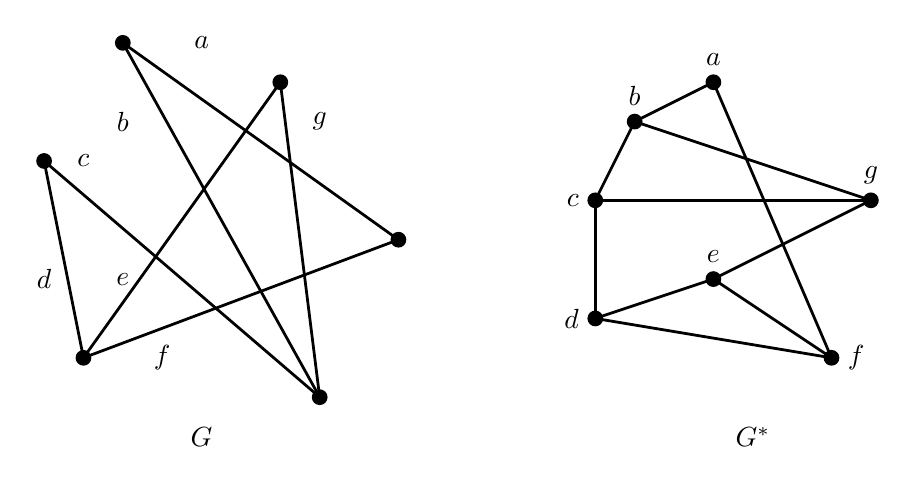
\begin{tikzpicture}
    \begin{pgfonlayer}{nodelayer}
        \node [BLACK_DOT] (1) at (-3.18182, 2.38636) {};
        \node [BLACK_DOT] (2) at (0.31818, -0.11364) {};
        \node [BLACK_DOT] (3) at (-4.18182, 0.88636) {};
        \node [BLACK_DOT] (4) at (-3.68182, -1.61364) {};
        \node [BLACK_DOT] (5) at (-1.18182, 1.88636) {};
        \node [BLACK_DOT] (6) at (-0.68182, -2.11364) {};
        \node [EMPTY] (7) at (-2.18182, -2.61364) {$G$};
        \node [EMPTY] (8) at (4.81818, -2.61364) {$G^*$};
        \node [label=above:{$a$}, BLACK_DOT] (9) at (4.31818, 1.88636) {};
        \node [label=above:{$b$}, BLACK_DOT] (10) at (3.31818, 1.38636) {};
        \node [label=left:{$c$}, BLACK_DOT] (11) at (2.81818, 0.38636) {};
        \node [label=left:{$d$}, BLACK_DOT] (12) at (2.81818, -1.11364) {};
        \node [label=above:{$e$}, BLACK_DOT] (13) at (4.31818, -0.61364) {};
        \node [label=above:{$g$}, BLACK_DOT] (14) at (6.31818, 0.38636) {};
        \node [label=right:{$f$}, BLACK_DOT] (15) at (5.81818, -1.61364) {};
        \node [EMPTY] (16) at (-2.18182, 2.38636) {$a$};
        \node [EMPTY] (17) at (-3.18182, 1.38636) {$b$};
        \node [EMPTY] (18) at (-3.68182, 0.88636) {$c$};
        \node [EMPTY] (19) at (-4.18182, -0.61364) {$d$};
        \node [EMPTY] (20) at (-3.18182, -0.61364) {$e$};
        \node [EMPTY] (21) at (-2.68182, -1.61364) {$f$};
        \node [EMPTY] (22) at (-0.68182, 1.38636) {$g$};
    \end{pgfonlayer}
    \begin{pgfonlayer}{edgelayer}
        \draw[EDGE] (4) to (3);
        \draw[EDGE] (6) to (3);
        \draw[EDGE] (4) to (5);
        \draw[EDGE] (6) to (5);
        \draw[EDGE] (4) to (2);
        \draw[EDGE] (2) to (1);
        \draw[EDGE] (1) to (6);
        \draw[EDGE] (9) to (10);
        \draw[EDGE] (9) to (15);
        \draw[EDGE] (10) to (11);
        \draw[EDGE] (10) to (14);
        \draw[EDGE] (11) to (12);
        \draw[EDGE] (11) to (14);
        \draw[EDGE] (12) to (13);
        \draw[EDGE] (12) to (15);
        \draw[EDGE] (13) to (15);
        \draw[EDGE] (13) to (14);
    \end{pgfonlayer}
\end{tikzpicture}

\endgroup
	\caption{Graph $G$ and its line graph $G^*$. The edges of $G$ and vertices of $G^*$ are labeled with the same alphabet.}
	\label{fig:line_graph_1}
\end{figure}

\begin{lemma}[Complexity and Vertex Order]\label{lem:contraction-vertex-order}
	Let $G$ be a graph and $G^*$ its line graph.
A edge in $G$, $e$, has a corresponding vertex in $G^*$, which we denote as $v_e$.
The number of edge neighbours of $e$ in $G$ precisely equals to the degree of vertex $v_e$ in $G^*$.
\end{lemma}
Therefore, using lemma \ref{lem:contraction-complexity} we see the cost of contracting a bond $e$ in $G$ is $O(d^{e+1})$.

If an edge $e$ is contracted in $G$, all the neighbouring edges of $e$ become neighbours of each other if they are not already.
The corresponding changes in its line graph $G^*$ is exactly simplicial elimination (Def \ref{def:simplicial_elimination}) of the vertex $v_e$ in $G^*$.
This process is demonstrated in figure \ref{fig:line_graph_simplicial_elimination}.
\begin{figure}[ht]
	\centering
	\resizebox{0.7\textwidth}{!}{
		% Graph Board TikZ export
% Exported: 2026-08-14T11:08:35.283Z
% Title: Untitled Graph
% Nodes: 41, Edges: 32

\begingroup
% --- Colors (define-if-not-already-defined) ---
\providecolor{zxRed}{RGB}{232,165,165}   % X spiders
\providecolor{zxGreen}{RGB}{216,248,216} % Z spiders
\providecolor{zxYellow}{RGB}{255,255,0}     % hadamard 
\providecolor{zxBlue}{RGB}{68,126,255}     % hadamard 


\tikzset{
    EMPTY/.style={minimum size=3.4mm,
        outer sep=-1.7mm},
    DOT/.style={inner sep=0mm, minimum size=3.4mm, shape=circle,
        draw=black, outer sep=-0.5mm, line width=1pt},
    BLACK_DOT/.style={minimum size=2mm, inner sep=0.3mm,
        outer sep=-0.15mm, fill=black, shape=circle},
    WORD_BALL/.style={draw=black, shape=rectangle, minimum size=6.5mm,
        rounded corners=3.2mm, inner sep=1.2mm, outer sep=-1.0mm,
        scale=1, font={\large\boldmath}, line width=1pt},
    GREEN_DOT/.style={DOT, fill=zxGreen},
    GREEN_WORD_BALL/.style={WORD_BALL, fill=zxGreen},
    RED_DOT/.style={DOT, fill=zxRed},
    RED_WORD_BALL/.style={GREEN_WORD_BALL, fill=zxRed},
    YELLOW_BOX/.style={fill=zxYellow, draw=black, line width=1pt, shape=rectangle, inner sep=0.6mm,
        minimum height=3.4mm, minimum width=3.4mm,
        font={\large\boldmath}},
    EDGE/.style={draw=black, line width=1pt},
    BLUE_DASHED_EDGE/.style={-, dashed, dash pattern=on 2pt off 0.5pt, ultra thick, zxBlue},
    GRAY_DASHED_EDGE/.style={-, dashed, dash pattern=on 3pt off 1.5pt, thick, lightgray}
}
\pgfdeclarelayer{edgelayer}
\pgfdeclarelayer{nodelayer}
\pgfsetlayers{edgelayer,nodelayer,main}

\begin{tikzpicture}
    \begin{pgfonlayer}{nodelayer}
        \node [BLACK_DOT] (1) at (-3.5122, 5.23171) {};
        \node [BLACK_DOT] (2) at (-0.0122, 2.73171) {};
        \node [BLACK_DOT] (3) at (-4.5122, 3.73171) {};
        \node [BLACK_DOT] (4) at (-4.0122, 1.23171) {};
        \node [BLACK_DOT] (5) at (-1.5122, 4.73171) {};
        \node [BLACK_DOT] (6) at (-1.0122, 0.73171) {};
        \node [label=above:{$a$}, RED_DOT] (7) at (3.9878, 4.73171) {};
        \node [label=above:{$b$}, BLACK_DOT] (8) at (2.9878, 4.23171) {};
        \node [label=left:{$c$}, BLACK_DOT] (9) at (2.4878, 3.23171) {};
        \node [label=left:{$d$}, BLACK_DOT] (10) at (2.4878, 1.73171) {};
        \node [label=above:{$e$}, BLACK_DOT] (11) at (3.9878, 2.23171) {};
        \node [label=above:{$g$}, BLACK_DOT] (12) at (5.9878, 3.23171) {};
        \node [label=right:{$f$}, BLACK_DOT] (13) at (5.4878, 1.23171) {};
        \node [EMPTY] (14) at (-2.5122, 5.23171) {$a$};
        \node [EMPTY] (15) at (-3.5122, 4.23171) {$b$};
        \node [EMPTY] (16) at (-4.0122, 3.73171) {$c$};
        \node [EMPTY] (17) at (-4.5122, 2.23171) {$d$};
        \node [EMPTY] (18) at (-3.5122, 2.23171) {$e$};
        \node [EMPTY] (19) at (-3.0122, 1.23171) {$f$};
        \node [EMPTY] (20) at (-1.0122, 4.23171) {$g$};
        \node [BLACK_DOT] (21) at (0.4878, -2.76829) {};
        \node [BLACK_DOT] (22) at (0.4878, -2.76829) {};
        \node [BLACK_DOT] (23) at (-4.0122, -1.76829) {};
        \node [BLACK_DOT] (24) at (-3.5122, -4.26829) {};
        \node [BLACK_DOT] (25) at (-1.0122, -0.76829) {};
        \node [BLACK_DOT] (26) at (-0.5122, -4.76829) {};
        \node [EMPTY] (27) at (-2.0122, -5.26829) {$G$};
        \node [EMPTY] (28) at (4.9878, -5.26829) {$G^*$};
        \node [label=above:{$b$}, BLACK_DOT] (29) at (3.4878, -1.26829) {};
        \node [label=left:{$c$}, BLACK_DOT] (30) at (2.9878, -2.26829) {};
        \node [label=left:{$d$}, BLACK_DOT] (31) at (2.9878, -3.76829) {};
        \node [label=above:{$e$}, BLACK_DOT] (32) at (4.4878, -3.26829) {};
        \node [label=above:{$g$}, BLACK_DOT] (33) at (6.4878, -2.26829) {};
        \node [label=right:{$f$}, BLACK_DOT] (34) at (5.9878, -4.26829) {};
        \node [EMPTY] (35) at (0.4878, -3.76829) {$b$};
        \node [EMPTY] (36) at (-3.5122, -1.76829) {$c$};
        \node [EMPTY] (37) at (-4.0122, -3.26829) {$d$};
        \node [EMPTY] (38) at (-3.0122, -3.26829) {$e$};
        \node [EMPTY] (39) at (-2.5122, -4.26829) {$f$};
        \node [EMPTY] (40) at (-0.5122, -1.26829) {$g$};
        \node [EMPTY] (41) at (0.9878, 0.23171) {$\bigg\downarrow$};
    \end{pgfonlayer}
    \begin{pgfonlayer}{edgelayer}
        \draw[EDGE] (4) to (3);
        \draw[EDGE] (6) to (3);
        \draw[EDGE] (4) to (5);
        \draw[EDGE] (6) to (5);
        \draw[EDGE] (4) to (2);
        \draw[BLUE_DASHED_EDGE] (2) to (1);
        \draw[EDGE] (1) to (6);
        \draw[EDGE] (7) to (8);
        \draw[EDGE] (7) to (13);
        \draw[EDGE] (8) to (9);
        \draw[EDGE] (8) to (12);
        \draw[EDGE] (9) to (10);
        \draw[EDGE] (9) to (12);
        \draw[EDGE] (10) to (11);
        \draw[EDGE] (10) to (13);
        \draw[EDGE] (11) to (13);
        \draw[EDGE] (11) to (12);
        \draw[EDGE] (24) to (23);
        \draw[EDGE] (26) to (23);
        \draw[EDGE] (24) to (25);
        \draw[EDGE] (26) to (25);
        \draw[EDGE] (24) to (22);
        \draw[EDGE] (21) to (26);
        \draw[EDGE] (29) to (30);
        \draw[EDGE] (29) to (33);
        \draw[EDGE] (30) to (31);
        \draw[EDGE] (30) to (33);
        \draw[EDGE] (31) to (32);
        \draw[EDGE] (31) to (34);
        \draw[EDGE] (32) to (34);
        \draw[EDGE] (32) to (33);
        \draw[EDGE] (29) to (34);
    \end{pgfonlayer}
\end{tikzpicture}

\endgroup
	}
	\caption{Contracting an edge $a$ (in dotted blue) in $G$ 
			makes all the neighbours of $v_e$ (labeled in red) in $G^*$ neighbours of each other.
			The cost of this contraction is $O(d^{3})$, as degree of $a$ in $G^*$ is two.
		}
	\label{fig:line_graph_simplicial_elimination}
\end{figure}

\begin{lemma}[Contracting Edge is Simplicial Elimination]\label{lem:contracting-makes-neighbours}
	Contracting an edge $e$ in a graph $G$ is equivalent to simplicially eliminating the corresponding vertex $v_e$ in the line graph $G^*$.
\end{lemma}

Therefore given any tree decomposition of $G^*$, we can find a simplicial elimination ordering $[v_{\alpha}, v_{\beta}, \cdots ]$ guaranteed by theorem \ref{thm:treewidth_triangulated_graph}.
The corresponding ordering of edges in $G$ $[\alpha, \beta, \cdots]$ is our desired contraction order. 
Each contraction will takes at most $O(d^{\text{tw}(G^*) + 1})$ time, and the total cost of contracting $G$ is $O(d^{\text{tw}(G^*) + 1})$.

\section{Miscellaneous Proofs}\label{sec:proofs}

\begin{proof}[Proof of Lemma \ref{lem:minor_treewidth}]
	We only need to prove that if a graph $G$ can be obtained from $H$ by performing one of the three graph-minor's operations, then the treewidth of $G$ is less than or equal to the treewidth of $H$. The lemma follows as any minor can be obtained by a finite sequence of these three operations.

	Let $T$ be a tree decomposition of $H$.
	We have three cases to consider.
	\begin{enumerate}
		\item If $G$ is obtained from $H$ by deleting an edge, then $T$ is also a tree decomposition of $G$. 
		\item If $G$ is obtained from $H$ by deleting a vertex $v$, let $T'$ be the tree decomposition of $G$ isomorphic to $T$ with $v$ removed from all bags. (We allow empty bags). It is clear that $T'$ is a tree decomposition of $G$ and the width of $T'$ is less than or equal to the width of $T$.
		\item If $G$ is obtained from $H$ by contracting an edge $(u, v)$. Let $w$ denote the new vertex after contraction. 
		Let $T'$ be the tree decomposition of $G$ isomorphic to $T$ with $u$ and $v$ replaced by a new vertex $w$ in all bags that contain $u$ or $v$. 
	\end{enumerate}

	In all cases, we can construct a tree decomposition of $G$ from a tree decomposition of $H$ with width less than or equal to the width of $T$. Therefore, the treewidth of $G$ is less than or equal to the treewidth of $H$.
\end{proof}

\begin{lemma}[Connection between Triangulated Graph and Cut Vertices]\label{lem:triangulated_cut_vertices}
	Let $G$ be a triangulated graph. Let $P$ be a cycle in $G$ and vertices $u, v \in G$ be a pair of non-adjacent vertices in $P$. 
	$u, v$ are cut vertices of $P$ (removing $u, v$ makes $P$ disconnected.) 
	Let $C_1, C_2$ be the two components of $P$ after removing $u, v$.
	If $C_1, C_2$ are not adjacent in $G$, then $u$ must be adjacent to $v$ in $G$.
\end{lemma}

\begin{proof}
	Provided $C_1, C_2$ are not adjacent in $G$, there must be a cycle of lenght four.
	If not, let $\mathcal{C}$ be the smallest cycle of $G$ that contain $u, v$.
	Since $G$ is triangulated, $\mathcal{C}$ must have a chord.
	This chord makes the cicle smaller, until the length of the cycle is four.
	See figure \ref{fig:triangulated_cycle} for an example of this process.

	\begin{figure}[ht]
		\centering
		% Graph Board TikZ export
% Exported: 2026-08-15T18:50:12.446Z
% Title: Untitled Graph
% Nodes: 19, Edges: 18

\begingroup
% --- Colors (define-if-not-already-defined) ---
\providecolor{zxRed}{RGB}{232,165,165}   % X spiders
\providecolor{zxGreen}{RGB}{216,248,216} % Z spiders
\providecolor{zxYellow}{RGB}{255,255,0}     % hadamard 
\providecolor{zxBlue}{RGB}{68,126,255}     % hadamard 


\tikzset{
    EMPTY/.style={minimum size=3.4mm,
        outer sep=-1.7mm},
    DOT/.style={inner sep=0mm, minimum size=3.4mm, shape=circle,
        draw=black, outer sep=-0.5mm, line width=1pt},
    BLACK_DOT/.style={minimum size=2mm, inner sep=0.3mm,
        outer sep=-0.15mm, fill=black, shape=circle},
    WORD_BALL/.style={draw=black, shape=rectangle, minimum size=6.5mm,
        rounded corners=3.2mm, inner sep=1.2mm, outer sep=-1.0mm,
        scale=1, font={\large\boldmath}, line width=1pt},
    GREEN_DOT/.style={DOT, fill=zxGreen},
    GREEN_WORD_BALL/.style={WORD_BALL, fill=zxGreen},
    RED_DOT/.style={DOT, fill=zxRed},
    RED_WORD_BALL/.style={GREEN_WORD_BALL, fill=zxRed},
    YELLOW_BOX/.style={fill=zxYellow, draw=black, line width=1pt, shape=rectangle, inner sep=0.6mm,
        minimum height=3.4mm, minimum width=3.4mm,
        font={\large\boldmath}},
    EDGE/.style={draw=black, line width=1pt},
    BLUE_DASHED_EDGE/.style={-, dashed, dash pattern=on 2pt off 0.5pt, ultra thick, zxBlue},
    GRAY_DASHED_EDGE/.style={-, dashed, dash pattern=on 3pt off 1.5pt, thick, lightgray}
}
\pgfdeclarelayer{edgelayer}
\pgfdeclarelayer{nodelayer}
\pgfsetlayers{edgelayer,nodelayer,main}

\begin{tikzpicture}
    \begin{pgfonlayer}{nodelayer}
        \node [label=above:{$u$}, BLACK_DOT] (1) at (0.65789, 0.81579) {};
        \node [BLACK_DOT] (2) at (-1.34211, 0.81579) {};
        \node [BLACK_DOT] (3) at (-1.84211, -1.18421) {};
        \node [EMPTY] (4) at (-4.34211, 1.81579) {};
        \node [EMPTY] (5) at (-0.34211, 1.81579) {};
        \node [EMPTY] (6) at (-0.34211, -2.18421) {};
        \node [EMPTY] (7) at (-4.34211, -2.18421) {};
        \node [BLACK_DOT] (8) at (-2.34211, 0.81579) {};
        \node [BLACK_DOT] (9) at (-2.34211, -1.18421) {};
        \node [label=below:{$v$}, BLACK_DOT] (10) at (0.65789, -1.68421) {};
        \node [BLACK_DOT] (11) at (2.65789, 0.31579) {};
        \node [BLACK_DOT] (12) at (2.65789, -1.68421) {};
        \node [EMPTY] (13) at (1.65789, 1.81579) {};
        \node [EMPTY] (14) at (4.65789, 1.81579) {};
        \node [EMPTY] (15) at (4.65789, -2.18421) {};
        \node [EMPTY] (16) at (1.65789, -2.18421) {};
        \node [EMPTY] (17) at (-1.84211, 2.31579) {$C_1$};
        \node [BLACK_DOT] (18) at (-3.34211, -0.18421) {};
        \node [EMPTY] (19) at (3.15789, 2.31579) {$C_2$};
    \end{pgfonlayer}
    \begin{pgfonlayer}{edgelayer}
        \draw[GRAY_DASHED_EDGE] (4) to (5);
        \draw[GRAY_DASHED_EDGE] (5) to (6);
        \draw[GRAY_DASHED_EDGE] (7) to (6);
        \draw[GRAY_DASHED_EDGE] (4) to (7);
        \draw[EDGE] (2) to (8);
        \draw[EDGE] (3) to (9);
        \draw[EDGE] (2) to (1);
        \draw[EDGE] (3) to (10);
        \draw[EDGE] (1) to (11);
        \draw[EDGE] (12) to (10);
        \draw[GRAY_DASHED_EDGE] (13) to (14);
        \draw[GRAY_DASHED_EDGE] (14) to (15);
        \draw[GRAY_DASHED_EDGE] (16) to (15);
        \draw[GRAY_DASHED_EDGE] (13) to (16);
        \draw[EDGE] (8) to (18);
        \draw[BLUE_DASHED_EDGE] (3) to (8);
        \draw[EDGE] (11) to (12);
        \draw[EDGE] (18) to (9);
    \end{pgfonlayer}
\end{tikzpicture}

\endgroup
		\caption{Provided $C_1$ and $C2_2$ are not adjacent, any chord in the cycle of lenght greater than 4, such as the one in dashed blue, will produce a smaller cycle that still contains $u$ and $v$.}
		\label{fig:triangulated_cycle}
	\end{figure}
	
	Let $\mathcal{C}$ be the length four cycle. There are two cases 
	\begin{enumerate}
		\item $u, v$ are adjacent in $\mathcal{C}$. Then we are done.
		\item $u, v$ are not adjacent in $\mathcal{C}$. Then the cycle must be of the form
		$[a, u, b, v]$, where $a \in C_1$ and $b \in C_2$. Since $a$ can not connect to $b$, $u$ must be adjacent to $v$.
	\end{enumerate}
\end{proof}

\begin{proof}[Proof of Lemma \ref{lem:simplicial_vertex}]
	We shall prove the following stronger statement. 

	\emph{
	For any triangulated graph $G$. Given any vertex $v \in G$, let $H$ be the set of vertices in $G$ that are farthest away from $v$. 
	Then there exists a simplicial vertex in $H$.
	}
	
	Recall that the distance between two vertices $u$ and $v$ in a graph is the length of the shortest path connecting them.

	The proof is by induction. 
	The base case is when $G$ has only one vertex $v$. This means $H = \{v\}$ and $v$ is simplicial.

	For a generic triangulated graph $G$ with a chosen vertex $v$, let $H_1$ be one of the connected components of $H$. Let $S$ be the set of vertices that are adjacent to $H_1$ and are not in $H_1$.
	See figure \ref{fig:simplicial_vertex} for a demonstration of this set up.

	\begin{figure}[ht]
		\centering
		% Graph Board TikZ export
% Exported: 2026-08-15T20:01:08.902Z
% Title: Untitled Graph
% Nodes: 27, Edges: 24

\begingroup
% --- Colors (define-if-not-already-defined) ---
\providecolor{zxRed}{RGB}{232,165,165}   % X spiders
\providecolor{zxGreen}{RGB}{216,248,216} % Z spiders
\providecolor{zxYellow}{RGB}{255,255,0}     % hadamard 
\providecolor{zxBlue}{RGB}{68,126,255}     % hadamard 


\tikzset{
    EMPTY/.style={minimum size=3.4mm,
        outer sep=-1.7mm},
    DOT/.style={inner sep=0mm, minimum size=3.4mm, shape=circle,
        draw=black, outer sep=-0.5mm, line width=1pt},
    BLACK_DOT/.style={minimum size=2mm, inner sep=0.3mm,
        outer sep=-0.15mm, fill=black, shape=circle},
    WORD_BALL/.style={draw=black, shape=rectangle, minimum size=6.5mm,
        rounded corners=3.2mm, inner sep=1.2mm, outer sep=-1.0mm,
        scale=1, font={\large\boldmath}, line width=1pt},
    GREEN_DOT/.style={DOT, fill=zxGreen},
    GREEN_WORD_BALL/.style={WORD_BALL, fill=zxGreen},
    RED_DOT/.style={DOT, fill=zxRed},
    RED_WORD_BALL/.style={GREEN_WORD_BALL, fill=zxRed},
    YELLOW_BOX/.style={fill=zxYellow, draw=black, line width=1pt, shape=rectangle, inner sep=0.6mm,
        minimum height=3.4mm, minimum width=3.4mm,
        font={\large\boldmath}},
    EDGE/.style={draw=black, line width=1pt},
    BLUE_DASHED_EDGE/.style={-, dashed, dash pattern=on 2pt off 0.5pt, ultra thick, zxBlue},
    GRAY_DASHED_EDGE/.style={-, dashed, dash pattern=on 3pt off 1.5pt, thick, lightgray}
}
\pgfdeclarelayer{edgelayer}
\pgfdeclarelayer{nodelayer}
\pgfsetlayers{edgelayer,nodelayer,main}

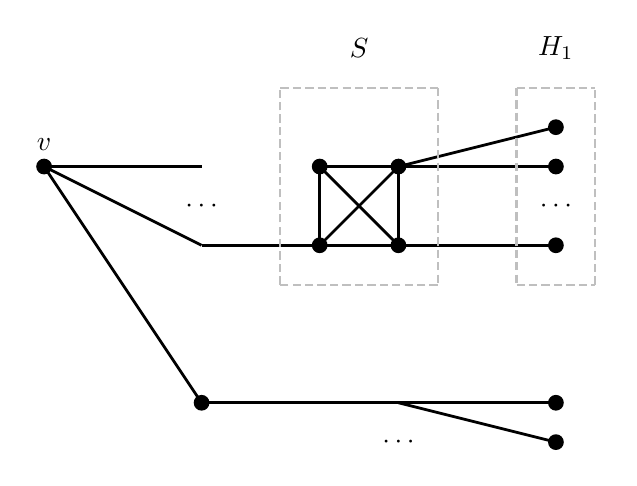
\begin{tikzpicture}
    \begin{pgfonlayer}{nodelayer}
        \node [label=above:{$v$}, BLACK_DOT] (1) at (-4.61111, 0.72222) {};
        \node [BLACK_DOT] (2) at (1.88889, 1.22222) {};
        \node [BLACK_DOT] (3) at (1.88889, 0.72222) {};
        \node [EMPTY] (4) at (1.88889, 0.22222) {$\cdots$};
        \node [BLACK_DOT] (5) at (1.88889, -0.27778) {};
        \node [BLACK_DOT] (6) at (1.88889, -2.27778) {};
        \node [BLACK_DOT] (7) at (1.88889, -2.77778) {};
        \node [BLACK_DOT] (8) at (-0.11111, 0.72222) {};
        \node [BLACK_DOT] (9) at (-1.11111, 0.72222) {};
        \node [BLACK_DOT] (10) at (-1.11111, -0.27778) {};
        \node [BLACK_DOT] (11) at (-0.11111, -0.27778) {};
        \node [EMPTY] (12) at (-2.61111, 0.72222) {};
        \node [EMPTY] (13) at (-2.61111, -0.27778) {};
        \node [EMPTY] (14) at (-2.61111, 0.22222) {$\cdots$};
        \node [EMPTY] (15) at (1.38889, 1.72222) {};
        \node [EMPTY] (16) at (1.38889, -0.77778) {};
        \node [EMPTY] (17) at (2.38889, -0.77778) {};
        \node [EMPTY] (18) at (2.38889, 1.72222) {};
        \node [EMPTY] (19) at (-1.61111, 1.72222) {};
        \node [EMPTY] (20) at (0.38889, -0.77778) {};
        \node [EMPTY] (21) at (-1.61111, -0.77778) {};
        \node [EMPTY] (22) at (0.38889, 1.72222) {};
        \node [BLACK_DOT] (23) at (-2.61111, -2.27778) {};
        \node [EMPTY] (24) at (-0.11111, -2.77778) {$\cdots$};
        \node [EMPTY] (25) at (-0.11111, -2.27778) {};
        \node [EMPTY] (26) at (1.88889, 2.22222) {$H_1$};
        \node [EMPTY] (27) at (-0.61111, 2.22222) {$S$};
    \end{pgfonlayer}
    \begin{pgfonlayer}{edgelayer}
        \draw[EDGE] (1) to (12);
        \draw[EDGE] (1) to (13);
        \draw[EDGE] (13) to (10);
        \draw[EDGE] (9) to (10);
        \draw[EDGE] (8) to (9);
        \draw[EDGE] (11) to (9);
        \draw[EDGE] (10) to (11);
        \draw[EDGE] (11) to (8);
        \draw[EDGE] (2) to (8);
        \draw[EDGE] (8) to (3);
        \draw[EDGE] (11) to (5);
        \draw[GRAY_DASHED_EDGE] (19) to (22);
        \draw[GRAY_DASHED_EDGE] (22) to (20);
        \draw[GRAY_DASHED_EDGE] (20) to (21);
        \draw[GRAY_DASHED_EDGE] (21) to (19);
        \draw[GRAY_DASHED_EDGE] (15) to (16);
        \draw[GRAY_DASHED_EDGE] (16) to (17);
        \draw[GRAY_DASHED_EDGE] (17) to (18);
        \draw[GRAY_DASHED_EDGE] (15) to (18);
        \draw[EDGE] (23) to (1);
        \draw[EDGE] (25) to (6);
        \draw[EDGE] (7) to (25);
        \draw[EDGE] (23) to (25);
        \draw[EDGE] (10) to (8);
    \end{pgfonlayer}
\end{tikzpicture}

\endgroup
		\caption{Demonstration of the proof of lemma \ref{lem:simplicial_vertex}. $H_1$ is a connected component of farthest vertices from $v$. $S$ is the set of vertices that are adjacent to $H_1$ and are not in $H_1$.
		}
		\label{fig:simplicial_vertex}
	\end{figure}
	I claim that $S$ is a clique.


	If $S$ contain only one vertex, there is nothing to prove.
	Assume $S$ contains at least two vertices. Let $u, w\in S$ be any distinct vertices.
	Both of $u, w$ are connected to $v$ via some vertices not in $H$, as they are closer to $v$. Both of them are also connected to some vertices in the connected component $H_1$.
	Note that no vertices in $H_1$ shall connected to any other vertices in closer to $v$ except those in $S$, as it will make the distance from $v$ to $H_1$ smaller.
	Therefore we are at the position to apply lemma \ref{lem:triangulated_cut_vertices} to the cycle formed by $u, w$ and any two vertices in $H_1$.
	In such way we have proved that any $u$ and $w \in S$ are adjacent, and therefore $S$ is a clique.

	Now apply the induction hypothesis to the subgraph induced by $H_1 \bigcup S$.
	If $H_1 \bigcup S$ is not a clique, then we can find a vertex $w \in H_1$ and $u \in S$ such that $w$ is distant 2 from $u$, and apply the induction hypothesis to the subgraph induced by $H_1 \bigcup S$ with $u$ as the chosen vertex states there is a simplicial vertex in $H_1$. 
	This vertex is also simplicial in $G$ as it is not adjacent to any vertices outside of $H_1 \bigcup S$.
	If $H_1 \bigcup S$ is a clique, then any vertex in $H_1$ is simplicial in $G$.
\end{proof}
